% P8 (project part) of the public test corpus (docs/DESIGN.md#testing). Written by the project; dedicated to the
% public domain (CC0 1.0). TikZ and pgfplots pictures of the kinds papers draw: a flow chart, a plot and a tree.
\documentclass[border=4pt]{standalone}
\usepackage{tikz}
\usepackage{pgfplots}
\pgfplotsset{compat=1.18}
\usetikzlibrary{arrows.meta,positioning,shapes.geometric}

\begin{document}
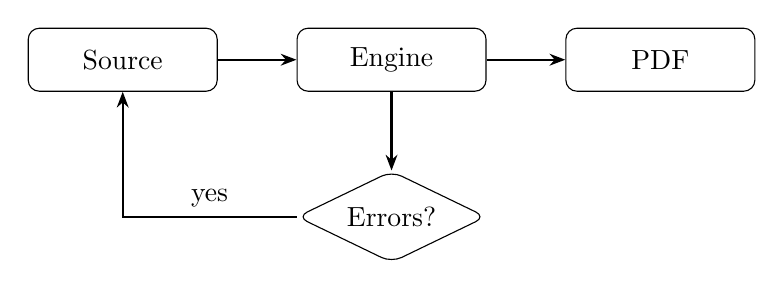
\begin{tikzpicture}[
  box/.style={draw, rounded corners, minimum width=2.4cm, minimum height=0.8cm, align=center},
  arrow/.style={-{Stealth[length=2mm]}, thick}]
  \node[box] (in) {Source};
  \node[box, right=1cm of in] (tex) {Engine};
  \node[box, right=1cm of tex] (pdf) {PDF};
  \node[box, diamond, aspect=2, below=1cm of tex] (err) {Errors?};
  \draw[arrow] (in) -- (tex);
  \draw[arrow] (tex) -- (pdf);
  \draw[arrow] (tex) -- (err);
  \draw[arrow] (err.west) -| node[pos=0.25, above] {yes} (in.south);
\end{tikzpicture}
\quad
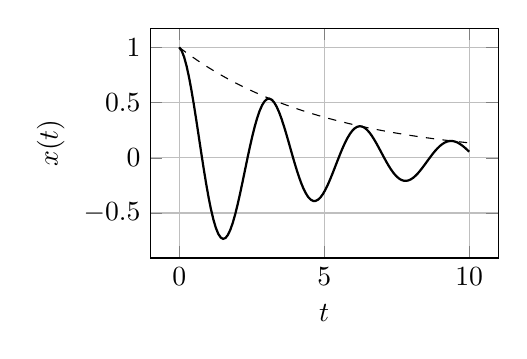
\begin{tikzpicture}
  \begin{axis}[width=6cm, height=4.5cm, xlabel={$t$}, ylabel={$x(t)$}, grid=major, samples=120, domain=0:10]
    \addplot[thick] {exp(-0.2*x)*cos(deg(2*x))};
    \addplot[dashed] {exp(-0.2*x)};
  \end{axis}
\end{tikzpicture}
\quad
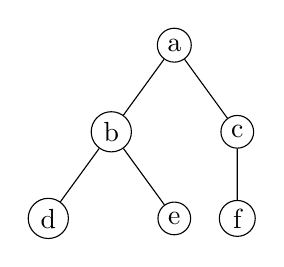
\begin{tikzpicture}[level distance=1.1cm, sibling distance=1.6cm, every node/.style={circle, draw, inner sep=2pt}]
  \node {a}
    child {node {b} child {node {d}} child {node {e}}}
    child {node {c} child {node {f}}};
\end{tikzpicture}
\end{document}
